\documentclass{article}
\usepackage{graphicx}
\usepackage{amsmath}
\usepackage{amssymb}
\usepackage{subfigure}
\usepackage{epstopdf}
\usepackage{setspace}
\usepackage{authblk}
\onehalfspacing
\newcommand{\nm}{\ensuremath{\,\textrm{nm}}}
\newcommand{\eV}{\ensuremath{\,\textrm{eV}}}
\newcommand{\uM}{\ensuremath{\,\mu\textrm{M}}}
\newcommand{\uW}{\ensuremath{\,\mu\textrm{W}}}
\newcommand{\meV}{\ensuremath{\,\textrm{meV}}}
\epstopdfsetup{update} % only regenerate pdf files when eps file is newer
\title{In situ tuning of nanorods' plasmon through etching with KCN}
%\author{Aquiles Carattino \and Saumya Khatua \and Michel
%Orrit}
\author[1]{Aquiles Carattino}
\author[2]{Saumyakanti Khatua}
\author[1]{Michel Orrit}
\affil[1]{Leiden Institute of Physics, Leiden, The Netherlands}
\affil[2]{Indian Institute of Technology- Gandhinagar, Ahmedabad,  India}
%\affil[3]{Leiden Institute of Physics, Leiden, The Netherlands}
%\ead{Corresponding Author Email Address}
%\cortext[a]{khatuask@iitgn.ac.in, Orrit@physics.leidenuniv.nl }
\begin{document}

\maketitle
\abstract{This is the abstract}

\section{Introduction}

Gold nanoparticles exhibit enhanced absoprtion and scattering cross sections
ranging from the visible to the near infra red. This property is closely related
to the surface plasmon (i.e. a collective oscilation of conduction electrons)
that in turn depends on the shape of the particles. For the case of gold
nanorods (AuNR) its surface plasmon resonance (SPR) energy depends on the aspect
ratio (AR) of the particle and can be found between $550\nm$ for
spheres (AR of $1$) to even above $800\nm$ for very elongated
particles.

The surface plasmon present great opportunities in (bio-)
sensing\cite{Zijlstra2012}, enhanced spectroscopies\cite{Sivapalan2013},
photothermal therapy\cite{Zhao2014}, and guiding light below the diffraction
limit. Success in many of these applications requires precise and in situ
control over the nanoparticles plasmon resonance energy. For example, maximum
fluorescence or Raman enhancement is achieved when the nanoparticle's plasmon
resonance is tuned to excitation laser wavelength or efficient
photothermal therapy requires nanoparticles' SPR to be tuned to NIR to
minimize the damage of healthy cells.

Typically, SPR is tuned by carefully manipulating the shapes of nanoparticles
during their synthesis. Particularly useful are the rod-shaped particles, whose
resonance can be tuned from $600\nm$ to over $1000\nm$ by changing their aspect
ratios through carefully adjusting the concentrations of gold-seed and silver
nitrate during the seed-mediated growth synthesis method. Many other
nanoparticles shapes, such as nanoprisms, nanorice, nanocubes, nanoshells, etc.
have been synthesized with their plasmon resonances covering entirely the
spectral range from visible to near-IR. Wet-chemical synthesis methods, however,
generally yield a broad distribution in nanoparticles sizes and/or shapes, which
hinders precise and reproducible tuning of nanoparticles SPR. Furthermore these
methods do not provide any in-situ adjustment of SPR; any change of which would
require a new synthesis.

Recently, new methods have been developed to tune nanoparticles' SPR after their
synthesis. These approaches can be divided in to two broad categories: ($1$) The
first group of methods tune the refractive index of the medium using an electric
or magnetic field. The advantage of these methods is that the SPR shift is
reproducible and reversible. However the tuning range is rather limited and the
continuous tuning within this range is difficult to achieve. ($2$) The other set
of approaches rely on controllably induce shape modifications of the
nanoparticles to tune the plasmon resonance through chemical or physical means.
For example, thermal reshaping was induced by illuminating the nanoparticles
with an intense, pulsed \cite{Link2000}\cite{Horiguchi2008} or continuous laser.
Chemical reshaping is also possible and was also the focus of several
studies\cite{Yuan2015} \cite{Carbo-Argibay2007} \cite{Rodriguez-Fernandez2005}
\cite{Jana2002}. In all these works a particular interest was put into the
surfactant employed to avoid the aggregation of the particles. The coating of
the surface will modify the heat transfer from gold to the medium (for the
thermal reshaping) and will cause that the reactivity of the sides and tips of
the particles to be different (for the chemical reshaping). This automatically
leads to an anisotropic reshaping, shortening the long axis or softening any
high-curvature region. Moreover, all the cited experiments were performed in 
bulk samples of nanorods in suspension. Single-particle experiments are however
scarce.

Another group has studied how the chemical reactivity of gold \cite{Ni2012} can
be altered by exploiting the plasmon resonance. This is achieved mainly through
changes in the surrounding temperature; it has to be noted that in these
experiments the surfactant was present as for the bulk experiments. In another
work\cite{Tsung2006}, high resolution TEM images allowed to show that the
crystal structure of individual particles is preserved after oxidation inducing
a shortening of the long axis of over $10\nm$. A common trend in the
vast majority of these works is that nanorods tend to reshape into spheres,
giving rise to a blue shift of the longitudinal plasmon resonance.

Here we present a new approach for precise and in situ tuning of plasmon
resonances of single gold nanorods isolated and immobilized over a glass
surface. A nanorod's plasmon resonance is tuned over $100\nm$ (starting from
$650\nm$ up to $780\nm$). Our method exploits well known chemistry between gold
and potassium cyanide (KCN), to controllably etch gold atoms from the
nanoparticle and thereby change its aspect ratio. We note that unlike many of
the previous studies, here we observe a red-shift of SPR on gold nanorods.
Our simulations based on the discrete dipole approximation method attributes
this red-shift to symmetric etching of gold nanorods from all sides resulting in
overall increase of aspect ratio. This is in contrary to previous studies, where
the etching was preferred at the tips, resulting in an overall decrease of
aspect ratios. The symmetric etching of gold nanorods is also verified from
scanning electron microscopy (SEM) images.

Our experiments are new in performing both single-particle studies while
removing the surfactant from the equation. Controlling the concentration of KCN
allows to fine tune the plasmon peak position of individual particles, without
hindering the known optical properties of them. Moreover we show that only a few
thousand molecules of KCN have to react with the nanoparticle in order to have
an observable change in the plasmon position.

%Give an overview of various
%chemicals used so far: H2O2 iron chloride, previous studies on cyanide? All
%these previous experiments were done in bulk solution of gold nanorods, which
%also contained large concentration of surfactants to prevent nanoparticles from
%aggregating and always yielded a blue-shift of plasmon resonance. The
%% blue-shift was rationalized from preferred etching of the tips than sides
%% because of less
%density of the surfactant on the tips.


%Many experiments that span from biosensing \cite{Zijlstra2012} to photodynamic
%therapy \cite{Zhao2014} and plasmon-enhanced spectroscopies
%% \cite{Sivapalan2013} highly depend on the position of the plasmon resonance.
%% Usually this is done at
%the moment of synthesis \cite{Gou2005}, by controlling the concentrations of
%growth and seed solutions. In this way is possible to induce the formation of
%longer or shorter particles \cite{Nikoobakht2003}. This methods however, always
%present a dispersion in the size distribution of the outcome, hindering the
%repeatability and the ability to build larger, periodic structures. Often an
%after-synthesis procedure is needed to achieve the needed parameters.

%Tuning the plasmon peak position after the synthesis has been object of several
%studies in the past. One of the possibilities is to achieve thermal reshaping
%that can be induced by illuminating the nanoparticles with an intense, pulsed
%laser\cite{Link2000}\cite{Horiguchi2008}. Chemical reshaping is also possible
%and was also the focus of several studies\cite{Yuan2015}
%\cite{Carbo-Argibay2007} \cite{Rodriguez-Fernandez2005} \cite{Jana2002}. In all
%these works a particular interest was put into the surfactant employed to avoid
%the aggregation of the particles. The coating of the surface will modify the
%heat transfer from gold to the medium (for the thermal reshaping) and will
%% cause that the reactivity of the sides and tips of the particles to be
%% different (for
%the chemical reshaping). This automatically leads to an anisotropic reshaping,
%shortening the long axis or softening any high-curvature region. Moreover, all
%the cited experiments are performed bulk samples of nanorods in suspension.
%Single-particle experiments are however scarce.


%The abundance of works in these topic is a good indication of the importance of
%having methods for altering the nanoparticle shape (and therefore their plasmon
%resonance) after the synthesis. It can also be stated that the next logical
%% step into the characterization of these methods are the single-particle
%% studies and
%the removal of the surfactant from the process. In this work we propose a
%chemical etching strategy that allows the in-\textit{situ} control of the
%plasmon resonance of single gold nanorods immobilized on a glass surface.

%We employ KCN as an etching agent; a known and well understood compound that is
%used not only in the nano-industry but also at bigger scales, for instance for
%gold mining. It's overall reaction formula is:
%\begin{equation*}
%4\textrm{Au} + 8\textrm{KCN}^-+\textrm{O}_2 + 2\textrm{H}_2\textrm{O}
%\leftrightarrows 4K\textrm{Au(CN)}_2^-+4\textrm{KOH}^-
%\end{equation*}
%In bulk this compound was used for reducing the aspect ratio of rods, i.e.
%blue shifting their plasmon \cite{Jana2002}. In a more recent paper it was also
%used for generating highly spherical particles with a narrow size
%distribution \cite{Lee2013}. 

% In our single-particle experiments of the AuNR show that by this reaction, it is
% possible to red-shift the plasmon resonance peak in more than
% $300\,\textrm{meV}$ (roughly $100\nm$ for particles starting with a
% SRP at $650\,\nm$) without degrading the shape or the optical properties
% of the nanorods, i.e. the rods preserve the rod-like geometry during the process
% and the FWHM of the peak follows the expected behaviour.
% 
% The preservation of the shape of the particles is confirmed by tracking the
% luminescence spectra of individual rods over time while the reactions is
% happening as well as by acquiring SEM images of the particles at defined
% intervals of the process. A simple model where etching is considered as being
% isotropic and constant (i.e. both the radius of the particle and it's length
% diminish at the same rate over time), yields a good agreement with both the
% plasmon shift and the changes observed in the FWHM. 
% 


\section{Experimental method}
\begin{figure}[p]
 \centering \includegraphics[width=0.95\linewidth]{Figures/01_Setup/setup_1.png}
 \caption{Schematic of the setup employed for acquiring luminescence spectra of
 singe gold nanorods. A) Schematic of the confocal microscope employed during
 the measurements. B) A typical 2-dimensional raster scan of the sample and C)
 the luminescence spectra of a single rod.}
 \label{fig:setup}
\end{figure}

Gold nanorods were synthesized by following standard seed-growth method (ref).
The average size of the nanorods was $60\nm\times 25\nm$ and their SPR is
located at $650\nm$ in water (SI figs: SEM image and bulk extinction of
nanorods as synthesized).

Single particle measurements were done on a home built confocal microscope
(Figure \ref{fig:setup}). A $532\nm$ laser was used for exciting the particles.
The excitation power was $300\uW$ at the back focal plane of the objective
(Olympus 60X NA 0.9 air). The luminescence signal was then filtered
with two $532\nm$ notch filters and was detected by either an avalanche
photodiode or a liquid nitrogen cooled CCD-spectrometer (Acton 500i).
The images were acquired by scanning the sample across a tightly focused laser
beam using a XYZ piezo scanning stage.

The samples were prepared by spin casting a suspension of AuNR on clean
coverslips and thoroughly rinsing them  with Milli-Q water and placed in an
ozone cleaner for eliminating the excess of CTAB. Afterwards the samples are
 placed in a flowcell; the initial spectra was taken with the rods immersed in
 Milli-Q water (see for example Figure \ref{fig:setup}.c). This initial characterization
allows to discard clusters of rods. Next, a solution of KCN was flowed into
the cell with concentrations ranging from $3\uM$ to $80\uM$.
In each case the spectra of approximately $10$ different particles is acquired
consecutively after focusing in each one. The time resolution varies according
to the exposure time and number of particles; in this work a spectra of each
particle is taken at least every minute.

% For confirming the preservation of the shape of the particles after the
% dissolution in KCN, SEM images are acquired. The samples are prepared by letting
% a droplet of a suspension of AuNR dry on top of a silicon wafer and then
% thoroughly rinsing them with Milli-Q water for eliminating the excess of CTAB.
% The same samples are employed for taking images before and after immersing the
% particles in $30\mu\textrm{M}$ KCN. For the analysis only the rods separated
% from each other are considered as to reproduce the conditions found in the
% optical experiment. After immersing the samples in KCN for a given period of
% time, they are rinsed with water to stop the reaction and dried with a nitrogen
% flow.
% 
% Bulk extinction spectra of the suspension of rods used previously is acquired as
% a function of time after a solution of KCN is added into the vial. This allows
% to compare single-particle experiments with previous results. 

\section{Results}

Figure \ref{fig:setup}.b shows a typical one-photon-excited luminescence image
of gold nanorods isolated on glass surface and covered with water.
Approximately, $90\%$ of the diffraction-limited bright spots originate from
single gold nanorods. This was confirmed by acquiring their luminescence
spectra, which show narrow Lorentzian lineshapes (ref). Figure \ref{fig:setup}.c
depicts a typical one-photon excited luminescence spectrum of a single gold
nanorod.

\begin{figure}[p]
 \centering 
 
\includegraphics[width=0.95\linewidth]{Figures/02_Experimental/Experimental.png}
 \caption{Single-photon luminescence spectra of gold nanorods immersed in $20\mu
 M$ KCN. A) Plasmon shift of a single rod. The curves are displayed at $70s$
 intervals. The insets display the intensity of the peak as a function of time
 and the resonance wavelength respectively. B) Shows the peak shift time-trace
 for 9 different particles. The red curve is the average while the green is
 the best fit from discrete dipole simulations with etching rate fixed at
 $1\nm/min$}
 \label{fig:plasmon_single_rod}
\end{figure}

Figure \ref{fig:plasmon_single_rod}.a shows the one-photon luminescence spectra
of a gold nanorod immersed in $20\uM$ KCN at intervals of $70\text{s}$. We
clearly observe a gradual red-shift of the nanorod�s plasmon resonance by
$100\nm$ over a time interval of $300$ seconds. This red-shift is also
associated with a decrease of intensity by factor of $4$. A more detailed
analysis shows that the nanorod�s plasmon resonance position (calculated from
fitting with a lorentzian function) varies almost linearly with respect to time
(inset of Figure \ref{fig:plasmon_single_rod}.a) We note the presence of an
additional shoulder peak at $650\nm$ ($1.9\,\eV$) that can be
observed for the less intense curves and is due to Raman scattering of water
that could not be completely removed when subtracting the background (see SI for
the spectra of the background).

We find the same trend for all the nanorods that were studied. Our results
are summarized in \ref{fig:plasmon_single_rod}.b, which shows the shift of
plasmon resonance wavelengths as a function of time for nine different rods (the
dashed lines). Each nanorod shows a shift of the plasmon resonance wavelength,
which varies almost linearly with time irrespective of their initial resonance
energy. The rate of SPR shift, however, varies significantly from particle to
particle with the fastest one being $15\nm/\textrm{minute}$ to the slowest one
of $2\nm/\textrm{minute}$. The red curve in the Figure is the average of all the
shifts; since the spectra of each particle were acquired at different instants,
we used a cubic spline for interpolating the values of the shift at given times.

The chemistry between gold and potassium cyanide is well known and well
understood; it is used not only in the nano-industry but also at bigger scales,
for instance for gold mining. Gold reacts with aqueous KCN in presence
oxygen to form $\textrm{Au(CN)}_2^-$, which is soluble in water. The reaction
can be written as follows
\begin{equation*}
4\textrm{Au} + 8\textrm{KCN}+\textrm{O}_2 + 2\textrm{H}_2\textrm{O}
\leftrightarrows 4K\textrm{Au(CN)}_2+4\textrm{KOH}
\end{equation*}
In our experiment, formation of $\textrm{Au(CN)}_2^-$ will result in etching of the gold
atoms from the nanorods, as has been reported previously.  

The etching of gold atoms from a nanorod has two effects: Firstly, the nanorod�s
volume will decrease gradually with longer reaction time. This is consistent
with our observation that the one-photon-luminescence intensity decreases with
time. Secondly, the aspect ratio of a nanorod can either decrease or increase
depending on the preferred direction of etching. Nanorods� aspect ratio will
decrease with time when the reaction happens preferably from the tips. This is
indeed the case for nanorods protected with CTAB and dispersed in solution. CTAB
binds weakly to the tips compared to the sides and therefore leaves the tips
more susceptible for chemical reactions (ref). The consequent decrease of aspect
ratio yields a blue shift of plasmon resonance (ref). In a second case, etching happens
isotropically from all sides and tips resulting in an overall increase of the
nanorod's aspect ratio. This is more likely scenario in our experiment as the
nanorods� surface does not have any protective CTAB.

Numerical Simulations based on the discrete dipole approximation model were
performed to further confirm that the red-shift of plasmon resonance is indeed
due to isotropic etching of the nanorods. The initial dimensions of the
particles are fixed at $25\nm\times60\nm$ which coincide with
the median dimensions of the distribution of sizes of the nanoparticles (see
SI). These simulations are carried on in steps of $0.5\nm$ for a total
of $10\textrm{nm}$ (i.e. the minimum particle size is $15\nm\times 50
\nm$). Figure \ref{fig:simulations}.a shows the scattering cross section
of the particle at different etching intervals. The observable red-shift is
comparable to the experimental one. The insets of the figure show the decrease
of the scattering peak value as well as the detailed time-evolution obtained
from the fitting of the peaks with a lorentzian function. Both are compatible
with the experimental observations. Furthermore it is possible to fix the
etching rate to best approximate the average plasmon shift. These results are
displayed as the green curve in Figure \ref{fig:plasmon_single_rod}.b. The best
approximation to the average is found when the etching rate is set to
$1\nm/\textrm{min}$. 

\begin{figure}[p]
 \centering
 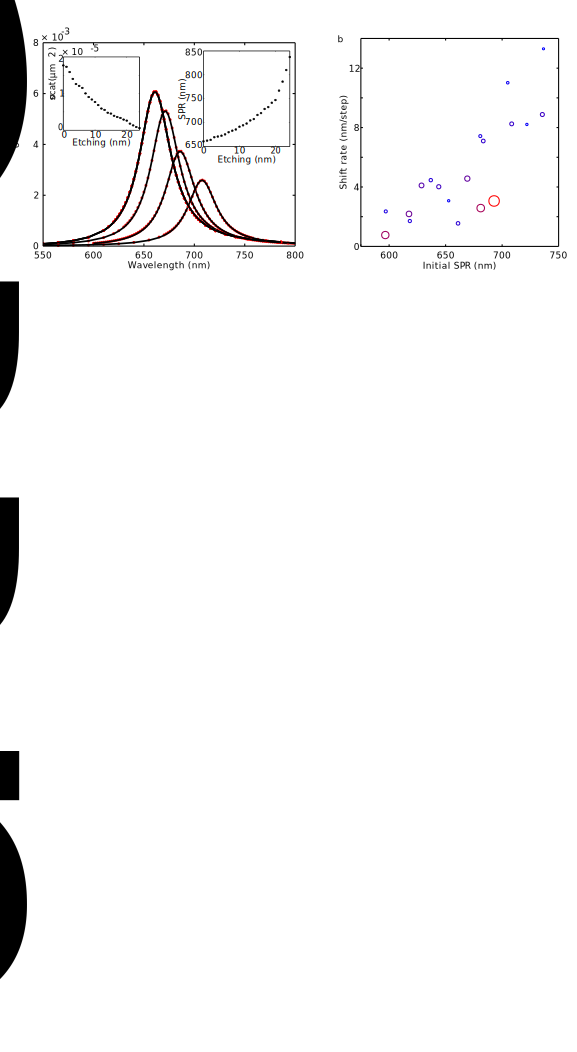
\includegraphics[width=0.95\linewidth]{Figures/02_Simulations/simulations.png}
 \caption{Simulated plasmon spectra at different etching steps. A) Examples of
 the curves obtained at different simulations steps. The black curves are
 fittings with lorentzians. The insets show the intensity and the SPR as a
 function of simulation step. B) Shows the shift rate as a function of the
 initial volume of the particle. C) Shift rate for particles with fixed width
 ($25\nm$) and variable length as a function of their initial SPR. }
 \label{fig:simulations}
\end{figure}

Furthemore the simulations allow to study the different shift rates that were
present in the experimental results. Figure \label{fig:simulations}.B shows the
different shift rates, as a function of the initial volume of the particles. The
shift rate is defined through a linear fit of the plasmon shift as a function of
etching steps. There is a great variability of results even for particles with
similar volumes. Figure \label{fig:simulations}.C shows the shift rate as a
function of initial SPR for particles with a fixed width ($25\nm$) and
different length. It can be seen that particles with higher aspect ratios
(higher SPR wavelengths) tend to shift more rapidly. This is also observed in
the inset of \label{fig:simulations}.A, where the shift as a function of
simulation step is clearly increasing more rapidly conform the etching
progresses. The simulations therefore prove that both the initial volume and SPR
will have a role in the rate at which the plasmon peak shifts. 

% \begin{figure}[p]
%  \centering
%  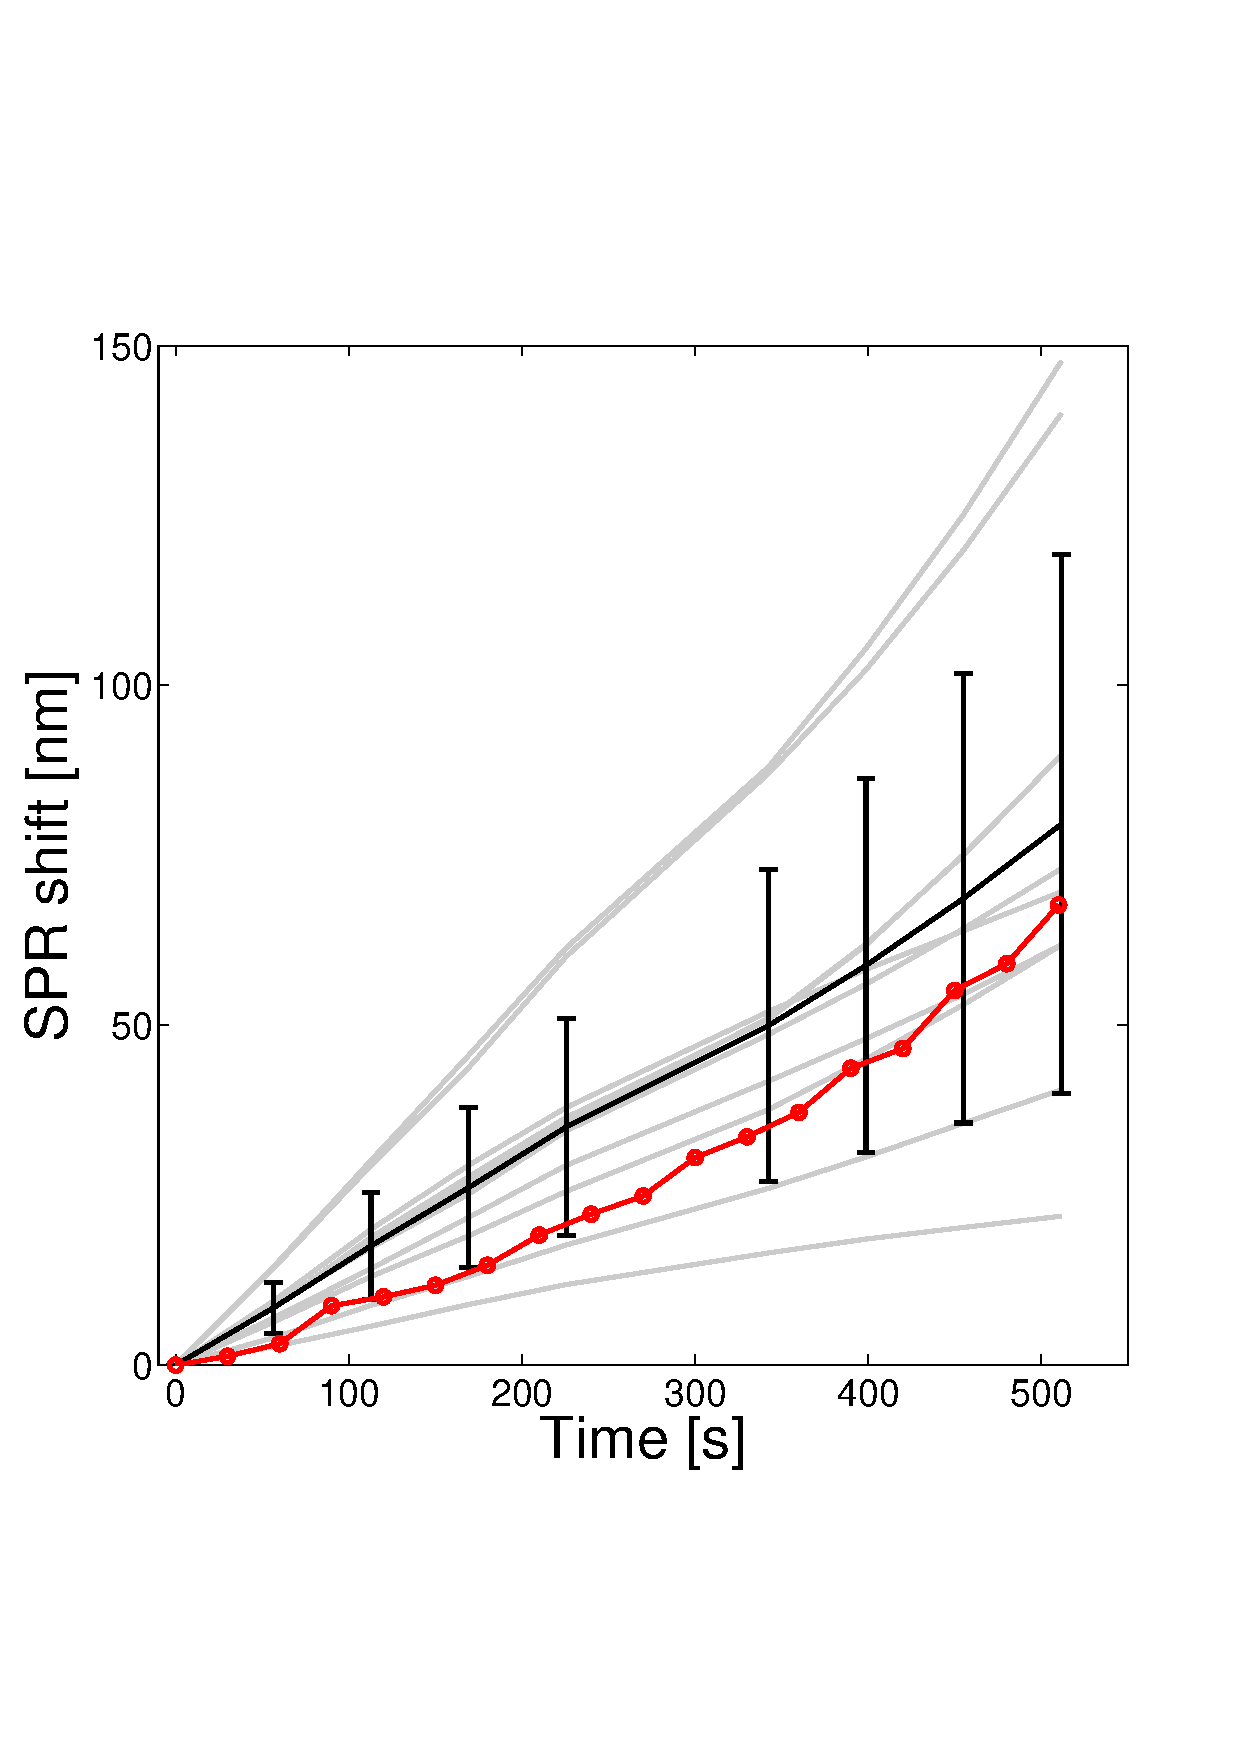
\includegraphics[width=0.95\linewidth]{plasmon_average.png}
%  \caption{Average plasmon shift (thick line) for 9 rods due to the etching with
%  $20\mu M$ KCN. The light curves are individual time traces while the thick one
%  is the average. The error bars are simply the standard deviation at each point. Over
%  time the peak distribution gets broader.}
%  \label{fig:plasmon_average}
% \end{figure}


% Figure \ref{fig:plasmon_average} shows the behaviour of the plasmon peak
% position for nine different rods while being etched with $20\,\mu\textrm{M}$
% KCN. The pale lines show each individual trace, while the darker is the average.
% The error bars are the standard deviation of the distribution at each point.
% Since spectra of different particles are taken at slightly different times (one
% after the other), an interpolation with cubic splines is used for calculating
% the average and the standard deviation at the given times. The bigger time step
% between $225\,\textrm{s}$ and $340\,\textrm{s}$ is due to an automatic
% refocusing happening on the particles every $5$ minutes. The plasmon shift of
% each particle ranges between $0.05\,\textrm{eV}$ and $0.35\,\textrm{eV}$ in over
% $9$ minutes. The dispersion of the rate change can be attributed to different
% initial aspect ratios. 

% \begin{figure}[p]
%  \centering
%  \includegraphics[width=0.95\linewidth]{shift_rate_vs_spr.png}
%  \caption{Different peak position shift rates as a function of initial plasmon
%  peak position.}
%  \label{fig:shift-vs-spr}
% \end{figure}
% 
% Figure \ref{fig:shift-vs-spr} shows the plasmon shift rate as a function of the
% initial plasmon peak position while immersed in $20\,\mu\textrm{M}$ KCN. The
% shift rate is extracted by a linear fit of the curves in Figure
% \ref{fig:plasmon_average}. The Figure shows a clear trend in which particles
% with lower aspect ratios (higher resonance energies) have a slower shift rate.
% The proposed model of isotropic etching fits this scenario, since particles
% closer to spheres change their aspect ratio much slower while reducing their
% axes at the same rate. Extracting the FWHM of each peak allows to determine that
% the optical and geometrical quality of the particles are being preserved during
% the experiment. 

\begin{figure}[p]
 \centering
 \includegraphics[width=0.95\linewidth]{Figures/03_Shifts/shifts.png}
 \caption{A) Plasmon FWHM of eight different particles immersed in $20\,\mu M$
 KCN as a function of their plasmon shift. The inset shows the results from the
 simulations carried on with the ADDA package. B) SPR Shift as a function of
 time for particles with the same initial SPR at different KCN concentrations.
 The inset shows the shift rate of these same particles.}
 \label{fig:FWHM}
\end{figure}

Figure \ref{fig:FWHM}.a shows how the FWHM of the plasmon decreases while the
shift increases. Mind the units of the plot, since it is not trivial the use of
wavelengths for the FWHM, we show these results in energy scale. At the
beginning of the reaction there is a rapid diminishing of the width, probably
due to the elimination of defects from the surface of the particles. Then a
minimum is reached for shifts between $75\nm$ and
$100\nm$. This decrease is explainable thinking that the higher
energy distance between the longitudinal plasmon peak and interband transitions
in gold makes less efficient the non radiative damping mechanisms in the
particles, hence yielding a narrower resonance as was already observed in other
studies\cite{Sonnichsen2002}. While the reaction continues, the width starts to
increase; this means that the reshaping at some point will start having an
effect on the shape of the particle and because of the reduction in particle
volume, other dephasing effects may start being relevant (for instance, surface
scattering). This is often encountered for shifts above $100\nm$, but
depends on the particle initial size and shape. The inset of the Figure shows
the FWHM obtained from the simulations. It is remarkable how similar the
simulations are to the experimental values.


% The inset in Figure \ref{fig:FWHM} shows the results of the
% ADDA\cite{Yurkin2011} simulations for a $25x60$nm particle while both its axis
% diminish evenly. The initial FWHM is $0.14\,\textrm{eV}$, slightly lower than
% the experimentally obtainable. This is due to particles not having a perfect rod
% shape or because of defects on their surface. The calculated width however
% diminishes to $0.1\,\textrm{eV}$ for shifts of just under $0.2\,\textrm{eV}$ as
% it is observed experimentally. This two results already show an agreement
% between a model of isotropic etching and our experimental results, and can be
% further confirmed by SEM images of the rods at different stages of the process.

% It is a known result that the cross section of the particle is proportional to
% its volume. Therefore a reduction of size will yield a reduction in intensity as
% is observed in all the performed experiments and simulations. Considering an
% atomic radius of gold of $144\,\textrm{pm}$(From Wikipedia. Better source?) the
% findings show an average etching rate of $1500$ atoms per second. The same trend 
% can also be observed for different concentrations of KCN, and therefore the
% number of reacting atoms per unit of time can also be changed.

Figure \ref{fig:FWHM}.b shows the plasmon peak shift as a function of KCN
concentration for particles with a plasmon peak position of roughly
$630\nm$. As shown for the simulations (Figure
\ref{fig:simulations}.C), the initial SPR will have a role on the etching rate,
therefore it is important to choose particles that are similar to each other.
The volume of the particles can be approximated by the intensity of the
luminescence, however is more prone to errors (different exitation intensities,
not perfectly focused on the particle, etc.) The timetraces of the peak position
clearly show that the shift rate is proportional to the concentration of KCN.
This result is also shown in the inset, where the shift rate is defined as
previously and plotted as a function of the concentration of KCN.

From these results and adapting the etching model it is possible to establish
that the reaction rate can be as low as $700$ atoms per second for a KCN concentration of
$10\mu M$. In the experiments performed at $3\mu M$ concentration, the particles
chosen didn't have a plasmon close to $630\nm$ and therefore are not
shown; if in any case the extrapolation still holds true for this low
concentrations it would yield a rate of just $200$ atoms per second. Inverting
the relationship, the plasmon peak shift while gold reacts with KCN happens at a
rate of roughly $0.5\cdot 10^{-6}\,\textrm{eV}/\textrm{atom}$.

% Every particle can be slightly different from another, not only because of its
% aspect ratio (and plasmon peak position) but also because of the presence of
% surface impurities. This was shown already in Figure \ref{fig:FWHM} where the
% FWHM decreases steeply at the beginning. The distribution of particle sizes and
% aspect ratios will in turn lead to different shift rates that will cause a
% broadening of the peak distribution after etching. These results are for
% particles immobilized on the coverslip and with all the surface capping washed
% out, leading to an isotropic etching. In bulk, where the rods are freely
% difussing and the surfactant is still present, the results are different.

Samples of the same nanorods are prepared for SEM imaging by drop casting the
same solution of rods. The images were acquired before the etching, after
$2\,\textrm{min}$ submersed in KCN and after $4\,\textrm{min}$. When particles
are isolated from each other, the model of the isotropic etching seems
appropriate, as the shape is preserved. It has to be noted, however, that for
aggregates of particles this no longer holds, and rods start to loose their
shape (see Supporting Information for SEM images.) Calculating the distribution
of sizes of the particles shows a slight increase in the aspect ratio but this
is however obscured by the broad distribution of values (even before starting
the etching). Averaging around $300$ different particles at each interval yields
an etching constant of $0.5\nm/\\textrm{minute}$, consistent with the optical
observations, not only of the plasmon shift but also of the diminishing
intensity as a function of time.

The presence of the surface is another aspect that may explain the difference
between the bulk and single-particle results. The surface would prevent the
reaction of gold with KCN from happening on one of the sides of the rods. By
definition this implies a non-isotropic model. On the other hand it would also
imply that the shape of the rods is not preserved since they would get
flattened. If this would be the case, the FWHM of the rods is expected to
increase but it was not observed, at least for the first couple hundreds
$\textrm{meV}$ of shift. The SEM images does not allow to assess this question
because there is no information on the third axis (perpendicular to the
surface). Experiments performed in an optical tweezer away from the surface as
done in Ref \cite{Ni2012} but without the capping agent would involve in
addition the use of microfluidics and therefore are much harder to perform.


%The same behaviour is observed for rods immersed in different concentrations of
%KCN, a red shift that can be of up to $100\,\textrm{nm}$. However the rate at
%which the plasmon shifts is different for different particles, as can already
%% be seen in Figure \ref{fig:plasmon_average}. It is expected that bigger
%% particles
%show a slower plasmon shift since the aspect ratio changes more slowly when
%reducing the axis length. For instance, a reduction of $1\,\textrm{nm}$ for a
%particle with axis $12.5\textrm{nm}\times30\textrm{nm}$ changes the aspect
%% ratio from  $2.40$ to $2.52$, while for a $25\textrm{nm}\times60\textrm{nm}$
%% the shift
%is to $2.46$. However there is no correlation between the initial brightness
%(proportional to the volume) and the observed rate. Different initial aspect
%ratios may also show different rates, but again no correlation is observed.
%% This means that there is an intrinsic property of the particles that makes
%% them react
%slower or faster with KCN. This is also confirmed by SEM images, since the
%distribution of longitudinal and transverse axis get broader over time.


%This can be further confirmed by SEM images of the rods.

%The study of the FWHM of the peak allows to confirm that during this process
% the optical properties of the plasmon do not get dampened.
%The red curve in the Figure is the result of the simulations that best fit the
%experimental results.

% \begin{figure}[p]
%  \centering
%  \includegraphics[width=0.95\linewidth]{Figures/shift_different_concentrations.png}
%  \caption{Plasmon shift of particles with a similar SPR peak at different
%  concentrations of KCN as a function of time.}
%  \label{fig:FWHM}
% \end{figure}
% 
% \begin{figure}[p]
%  \centering
%  \includegraphics[width=0.95\linewidth]{Figures/shift_rate_vs_spr.png}
%  \caption{Plasmon shift rate of particles with different initial plasmon peak
%  positions when immersed in $20\mu M$ KCN.}
%  \label{fig:FWHM}
% \end{figure}

% \begin{figure}[p]
%  \centering 
%  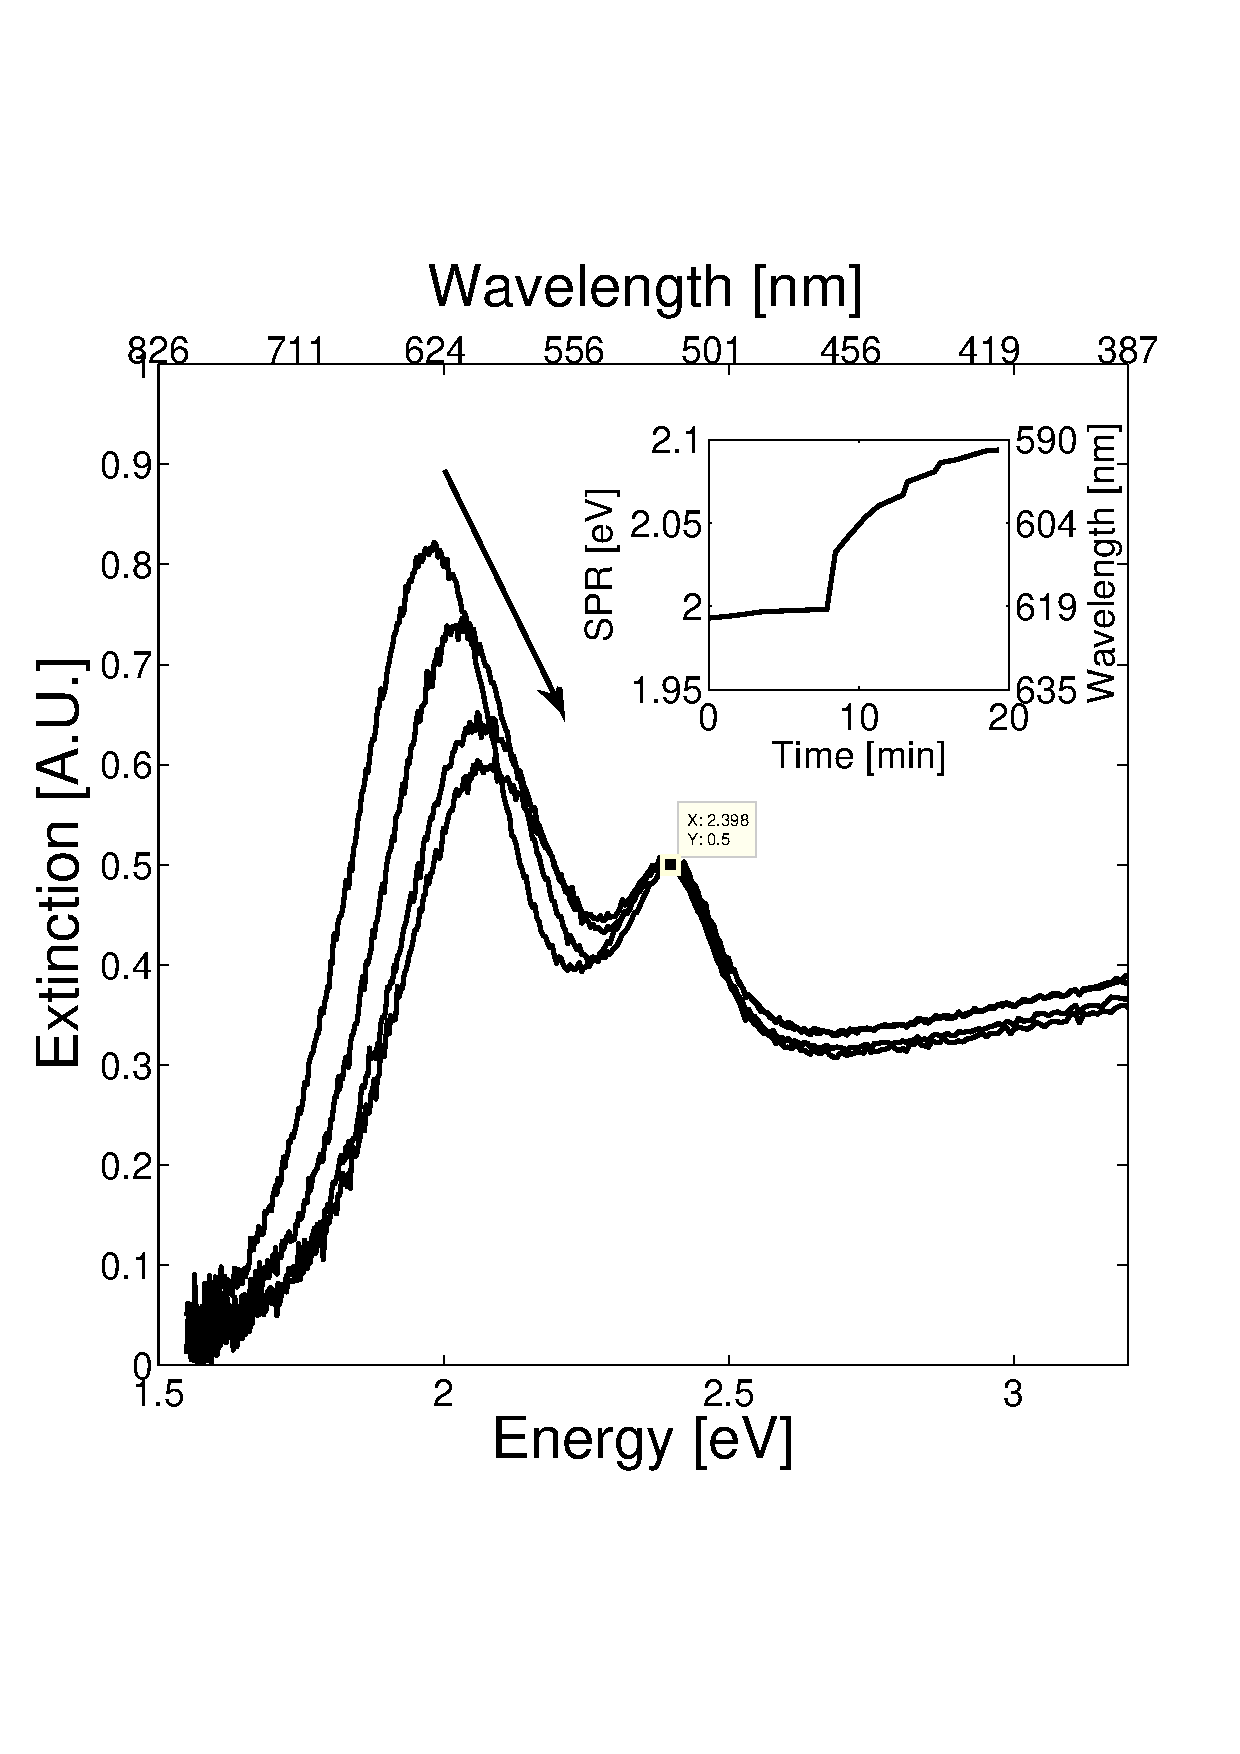
\includegraphics[width=0.95\linewidth]{Figures/plasmon_bulk.png}
%  \caption{Bulk extinction spectra at $10$ minutes time-interval. The arrow
%  indicates the time evolution. A solution of KCN is added into the cuvette with
%  the nanorod suspension as to have a $50\,\mu M$ concentration for the first 9
%  minutes; then this step is repeated, yielding a final KCN concentration of
%  $100\, \mu M$. The inset shows the peak position of the SPR position as a
%  function of time, extracted by fitting the spectra with a lorentzian.  }
%  \label{fig:bulk}
% \end{figure}
% 
% Figure \ref{fig:bulk} shows a blue-shift of the longitudinal plasmon peak for a
% suspension of rods while being etched with KCN; these results were already
% reported in several works and under different
% conditions\cite{Rodriguez-Fernandez2005}\cite{Tsung2006}\cite{Jana2002}. The
% spectra is plotted at intervals of $9$ minutes after adding a solution of KCN
% that results in a concentration of $100\mu\textrm{M}$ in the vial. All spectra
% plots are normalized to the transverse plasmon peak at $2.4\,\textrm{eV}$ for increasing
% the visibility of the longitudinal plasmon shift. These results are strikingly
% different from the single-particle measurements and can be explained by the
% protective bilayer of CTAB present.
% 
% The plasmon peak position shifts towards higher energies (from approximately
% $2.0\,\textrm{eV}$ to $2.1\,\textrm{eV}$ or equivalently from $620\,\textrm{nm}$
% to $592\,\textrm{nm}$). It means that the rods are reshaping into spheres as was
% previously observed \cite{Jana2002}. This implies that the tips of the rods are
% more exposed to KCN than the sides as is expected from the their higher
% curvature\cite{Yuan2015}. 
\section{Conclusions}
In this work we have shown a simple method that allows the tuning of the plasmon
peak position of single gold nanorods with nanometer accuracy and over the range
of $100\nm$ ($300\meV$). More importantly, it is shown that
the rodlike shape is preserved for these shifts and therefore the well known
optical properties of the nanoparticles are not dampened. Moreover the absence
of the capping agent also works in favor of the proposed mechanisms in previous
works.

The experiments allow to record the plasmon peak with a relatively high temporal
and spectral accuracy, allowing to stop the reaction when the resonance is at
the desired value. Both SEM images and the study of the FWHM of the longitudinal
resonance allow to confirm that the shape of the rods is being preserved. The
agreement between the simulations assuming an isotropic etching and the
experimental results not only shows the link between both measurements but also
provide a way of predicting the behaviour of the plasmon peak for different
rods.

It is also found a great distribution of the rate at which the plasmon peak
shifts for different particles under the same experimental conditions. This can
be attributed to the initial aspect ratios of each particle. Sphere-like
particles will show a small shift due to the fact that the aspect ratio is
constant while under isotropic etching. The more elongated particles, on the
other hand, will have a much steeper increase in aspect ratio while being
etched. The majority of the rods present in the samples studied belong to an
intermediate position, with their resonance at $650\nm$ (aspect ratio
of $2.4$). The simulations agree with this statement, however experimental date
to further confirm this hypothesis is needed. 

% only considering that there is an intrinsic difference between particles; this
% differences can be attributed to defects on the particle surface or to
% inhomogeneities in the left over CTAB capping the rods even if care is taken to
% remove it by rinsing with water. Different initial conditions (such as initial
% aspect ratio or volume) are considered but no correlation with the rate of the
% shift is observed. This doesn't discard any relationship between them as there
% can be an interwined dependence on both initial size and aspect ratio.
% Experiments on larger ensembles of particles would increase the possibility of
% finding more nanorods with the same initial conditions.

The role of the capping agent has largely been studied and has always been held
responsible for the observations both in chemical etching\cite{Yuan2015} and for
photothermal reshaping\cite{Horiguchi2008}. Avoiding the presence of the
passivating layers is impossible in suspension, since gold nanoparticles would
aggregate. Our results do not only provide a method for changing the plasmon
resonance after the synthesis and in-situ, but also provide evidence that
supports previous observations regarding the effect of the curvature and the
accessibility of KCN to the surface of the particle. We also show that
single-particle experiments open new ways of controlling the particle shape.

A simple approximation of the reaction rates show that the dissolution of just a
few thousand atoms in the gold nanoparticle are enough for detecting a change in the
luminescence spectra. This method is not aimed at pushing the detection limits
of KCN (or other substances) via plasmonic structures, but still has proven to
be highly efficient. A better approach to sense plasmon shifts is to detect
changes in the cross section at the plasmon wing (via scattering or
photothermal detection, for instance). 

The report by Wei et Al. in 2012 \cite{Wei2012} shows these ideas but in a
slightly different condition. They found sensitivities to the presence of KCN in
the order of the nM. We have readily approached this threshold and believe that
the sensitivity of single particles to very low concentrations (in the order or
below the nM) should be higher, specially if using smaller particles with a
higher aspect ratio.

Combining this results with the catalytic properties of gold and the presence of
the plasmon resonance opens the door for fine-controlling chemical reactions
while irradiating the particles with specific wavelengths. Using a compound with
a lower reactivity with gold would allow to compare the difference of reaction
rates while exciting or not the longitudinal plasmon and are already a work in
progress in our lab.

\bibliography{bibliography}{}
\bibliographystyle{ieeetr}

\end{document}
